\fancyhead[LO, RE]{Exploitation du contenu}

Avant d'arriver à la finalité de notre projet, il est essentiel d'explorer tous les textes que nous avons à disposition et pas seulement le corpus enrichi que nous venons de mettre en place. Cela nous permet de récupérer de plus amples informations sur le texte et sa composition, afin d'étudier son contenu mais aussi trouver les meilleurs moyens d'analyse de corpus pour créer notre alignement\index{Alignement}. Nous pouvons ainsi déjà nous avancer sur notre objectif en travaillant notamment le lexique des chapitres, mais aussi les différences entre les chapitres et entre les langues, travail qui est au c\oe ur de notre analyse du \emph{Traité\index{Traite des delits et des peines@Traité des délits et des peines}} de Beccaria. Notre démarche consistera donc à expliquer la manière dont s'étudie un texte par les statistiques, puis à introduire deux modules pour effectuer cette exploration et enfin présenter plusieurs fonctionnalités pour dégager diverses données à propos des textes de notre corpus. 

\section{L'analyse statistique des données textuelles\index{Statistique textuelle}, une autre manière d'étudier un corpus}
Afin d'étendre le domaine de l'étude de texte, il est essentiel de trouver de nouvelles manières d'explorer complètement un corpus. Pour se faire, il est intéressant de se tourner vers d'autres disciplines, de manière à combiner notre propre champ d'études avec d'autres probablement plus inattendus. C'est ainsi que s'est développée l'analyse statistique des données textuelles, mêlant l'étude de texte à des mathématiques.

\subsection{Des mathématiques pour réaliser une analyse textuelle}
La statistique textuelle est une méthode qui se trouve à la croisée de plusieurs disciplines et tient son origine du développement d'un nouveau moyen d'analyse de texte, qui utilise les mathématiques. Diverses recherches ont été effectuées sur des textes et des ouvrages en prenant en compte des éléments statistiques, tels que des fréquences et des cooccurrences et plusieurs lois de probabilité ont alors été énoncées. La première et plus importante est la loi d'Estoup-Zipf, plus tard devenue loi de Zipf-Mandelbrod. Elle porte sur la fréquence d'un mot dans un texte et montre que cela suit un schéma, où le rang du mot dépend du nombre de fois où il apparaît dans le texte. Ce schéma a été déterminé après l'observation de l'ouvrage de James Joyce, \emph{Ulysse}. En comptant les occurences de mots, Zipf a découvert que le mot le plus courant revenait 8 000 fois, le dixième 800 fois, le centième 80 fois et le millième 8 fois, ce qui lui a inspiré la loi. Cette loi a ensuite été peaufinée par le mathématicien français Benoît Mandelbrot, qui a rajouté un coefficient, qui ira prendre en compte les mots-vides qui sont les mots très fréquents qui faussent la courbe. Il a également rajouté deux paramètres, à savoir le type de texte et la langue étudiée, afin que la loi puisse s'adapter. Cette correction a permis de parfaire le résultat, qui est alors exact, et cette loi a ouvert la voie ensuite à de multiples autres lois ou formules mathématiques qui s'appliquent à l'analyse d'un texte. Dans ce cadre, nous pouvons citer la loi de Heaps qui s'interroge sur la probabilité de l'apparition d'un nouveau mot dans un texte et la contagion qui est la probabilité qu'un mot réapparaisse après l'avoir vu une première fois. Ces deux méthodes peuvent se lier entre elles puisqu'il peut être intéressant d'étudier si un mot apparaîtra et ensuite combien de fois il le fait. Ces méthodes statistiques ont par la suite été étendues pour une étude multi corpus, comme avec la boite à moustache qui s'intéresse à l'apparition du mot à travers plusieurs textes (minimum, maximum, quart 1, quart 3 et médiane). La répartition qui sera donnée avec la boîte à moustache permettra de savoir s'il y a une spécificité en fonction d'un texte du corpus, si un mot est plus utilisé dans un des textes que dans un autre. Cela a, par exemple, été utilisé avec des \oe uvres de théâtres de quatre auteurs~: Pierre et Thomas Corneille, Molière et Scarron. La recherche s'est faite sur la fréquence d'apparition d'un mot choisi au préalable dans tous les textes de ces auteurs.

Ces méthodes ont par la suite été perfectionnées, augmentées et développées de manière à être plus accessibles et plus aisées d'utilisation pour les historiens, les linguistes et d'autres praticiens des sciences sociales, les mathématiques brutes n'étant pas toujours facilement exploitables.

\subsection{Une abondance d'outils pour opérer l'analyse statistique des données\index{Statistique textuelle}}
L'essor de l'informatique dans les disciplines des sciences sociales et des lettres a permis le développement de nouvelles techniques et notamment la mise en place d'outils pour traiter les données textuelles. Il y en a eu un très grand nombre de créés qui n'ont pas tous la même fonction, ni le même angle de travail, en fonction de leur approche du corpus de texte et des méthodes statistiques. Si la démarche n’est pas la même, les procédures se ressemblent, telles que le calcul de spécificité lexicale ou l’analyse des concordances\footcite[p.~33-36]{stat_text_garnier}. La forme sous laquelle se présente le corpus est également importante et l’une des plus significatives, qui sera également essentielle dans notre travail, est la lemmatisation. Elle consiste à regrouper des mots selon une forme plus basique et ainsi à \og~ ramener un verbe conjugué à son infinitif, rassembler les formes au pluriel et au singulier, les masculins et féminins, et plus généralement regrouper les formes qui correspondent à une même racine, avec des désinences différentes\footcite[p.~867]{stat_text_guerin}.~\fg{}. La lemmatisation est utilisée et favorisée par la majorité de ceux qui effectuent les statistiques textuelles\index{Statistique textuelle} et elle est ainsi parfois insérée directement lors de l'import d'un corpus en fonction de l'outil à disposition, ce qui permet d'avoir plus de résultats d'analyse lors des recherches sur le logiciel.

Il existe un certain nombre de logiciels de statistiques textuelles\index{Statistique textuelle} et même si une concurrence existe, ils sont assez variés pour que certains soient plus aisés à utiliser selon le type de corpus qui est soumis. Parmi ceux-ci, nous pouvons en citer trois de références~: \textsc{spad} (Système Portable pour l'Analyse des Données Textuelles) contient un module spécifique dédié aux données textuelles et est davantage adapté aux textes courts~; \textsc{alceste} (Analyse des Lexèmes Cooccurrents dans les Énoncés Simples d'un Texte) a été conçu pour le traitement des données textuelles et pour des corpus de taille plutôt importante~; \textsc{lexico} est assez proche de \textsc{spad} et possède une interface avant tout visuelle\footcite[p.~33-36]{stat_text_garnier}. Ces trois logiciels possèdent tous une lemmatisation automatique qui est parfois assistée d'options plus avancées. Parmi les autres logiciels, nous pouvons également mentionner le logiciel \textsc{rstudio} qui fait du comptage de mots mais qui est principalement un logiciel statistique et graphique s'appuyant beaucoup sur de la programmation. Plus récemment, en 2010, une nouvelle plateforme logicielle en open-source a fait son apparition~: \textsc{txm}\footcite{txm_plateforme}. \textsc{txm} offre des fonctionnalités similaires aux logiciels précédemment cités, certaines des requêtes peuvent d'ailleurs être faites avec le langage de programme \textsc{r}, qui fait tourner le logiciel \textsc{rstudio} et offre également la possibilité de produire le corpus sous de nombreuses formes (\textsc{txt}, \textsc{doc}, \textsc{odt} ou encore \textsc{xml-tei}). Ce logiciel opère une lemmatisation automatique, qu'il est possible d'utiliser par la suite pour les requêtes et permet également d'effectuer ses propres annotations sur le corpus à disposition.

Ainsi, ces divers logiciels rendent possible un travail plus aisé selon le corpus qu'il faut manipuler et encouragent une diversité d'analyses sur un corpus, car cela peut alors faire ressortir des informations ou des données que d'autres types d'analyses n'auraient pas relevées.  Dans le cadre de notre étude de texte, le choix de logiciels s'est porté sur \textsc{txm} et \textsc{rstudio}, avec lesquels nous allons effectuer diverses analyses pour explorer notre corpus.

\section{Analyser les textes de notre corpus~: import et manipulation à l'aide de logiciels de statistiques textuelles\index{Statistique textuelle}}
Avant de pouvoir réaliser nos analyses avec \textsc{txm} et \textsc{rstudio}, il est nécessaire d'importer le corpus sur chacun des logiciels et d'apporter certains éléments, dont notamment un fichier de métadonnées, de manière à pouvoir ensuite travailler avec les textes à disposition. Cet import sera différent en fonction des logiciels, du fait de leurs caractéristiques propres.

\subsection{TXM~: un import simple et rapide, dépendant du type de fichier}
Notre travail avec \textsc{txm} s'effectue en deux temps et avec deux formes différentes du corpus. Cela nécessite donc deux imports distincts, qui ne solliciteront pas les mêmes éléments et ne demanderont pas la même charge de travail.

Dans un premier temps, il est nécessaire d'effectuer un import simple du corpus par langue et avec les divers chapitres que nous avons océrisés\index{OCR!ocerisation@océrisation}, mis en forme et corrigés. Ces fichiers, existant au format \textsc{txt}, ne nécessitent qu'un élément supplémentaire afin de pouvoir être importé sur le logiciel \textsc{txm}~: un fichier de métadonnées. Effectivement, l'interface \textsc{txm} possède plusieurs styles d'import et les fichiers de textes brut ou fichier word et certains fichiers en \textsc{xml} demandent un \textsc{csv}, qui contiendra les informations sur l'identifiant du document importé, ainsi que sa langue et sa date, dans l'intention d'avoir des données précises lorsqu'elle créera le corpus que nous manipulerons. L'identification de ces données lui permettra ensuite de trier nos documents grâce à ces métadonnées, pour créer des sous-corpus, des partitions ou établir certaines statistiques suivant ces critères. Une fois que le fichier \textsc{csv} contient les métadonnées correspondant au corpus soumis, il est possible d'importer ce corpus et \textsc{txm} peut ensuite procéder à diverses opérations avec les textes fournis.

Extérieurement, le logiciel \textsc{txm} ne semble procéder qu'à un import de corpus que nous pouvons ensuite utiliser. Intérieurement, il effectue de nombreuses opérations qui visent à présenter le texte sous de nouvelles formes et avec de nouveaux encodages, afin de maximiser les capacités d'analyse. L'une de ces modifications principales, que nous avons longuement étudiée dans le chapitre précédent, vise à modifier le texte afin qu'il soit encodé au format \textsc{xml-tei} et balisé mot par mot, avec un enrichissement pour chacun des mots d'attributs sur sa catégorie grammaticale et lexicale, offrant ainsi plus de statistiques, sur des données inédites. C'est ce type de fichier que nous utiliserons dans un deuxième temps et cette fois-ci en effectuant un import de corpus multilingue\index{Alignement!corpus multilingue}. Comme nous l'avons expliqué dans le chapitre \ref{chap_annotations}, nous avons modifié ce fichier encodé en intégrant de nouvelles balises, dont notamment une avec un attribut \textit{mlx} qui relève les mots du texte qui contiennent des termes juridiques, fil conducteur de notre analyse dans notre objectif d'alignement\index{Alignement}. Ainsi, une fois les fichiers modifiés pour contenir les nouvelles balises, nous allons pouvoir les importer sur le logiciel \textsc{txm} puisque ce dernier possède également un mode d'import pour ces types de fichiers~: \textsc{xml-tei txm}. Cette fonction permet en résumé de réimporter dans le logiciel un texte qu'il a lui-même balisé avec des attributs qui contiennent l'information que le document a été encodé par \textsc{txm} (exemple~: \mintinline{xml}{<txm:ana resp="#txm" type="#frpos">}). À partir de là, il est important de vérifier la langue que le logiciel choisira pour importer le corpus. Il est possible de lui imposer de deviner la langue du texte. Cette fonctionnalité est disponible à chaque import de corpus mais n'aurait pas fait sens lors du premier import que nous avons mentionné, puisque, ici, nous avons un moyen de rechercher des informations à travers un corpus multilingue\index{Alignement!corpus multilingue}, ce qui n'était pas le cas lorsque les documents étaient seulement des fichiers .txt. En devinant la langue du corpus, il prend en compte les distinctions qu'auront les textes vis-à-vis de leur attribut mais pourra tout de même les traiter comme un tout. Il sera possible de travailler selon ces spécificités ou selon les caractéristiques communes à tous les textes.

Il est donc possible avec \textsc{txm} d'étudier des textes sous différents formats, diverses langues ou avec plusieurs annotations pour explorer au mieux le texte grâce à la multitude de fonctionnalités proposées. Nous pourrons observer les différents résultats que nous obtenons à propos de notre corpus et nous aurons notamment la possibilité de les comparer avec ceux que produit \textsc{rstudio}, avec le même corpus qui doit également être importé sur ce logiciel.

\subsection{RSTUDIO~: un import par de la programmation}
\textsc{rstudio} fonctionne à partir du langage de programmation \textsc{r}, qui est destiné aux statistiques et aux graphiques. Son environnement de développement intégré (IDE) propose de travailler avec une console et un terminal ainsi qu'en lien avec notre bureau~; l'import du corpus, de même que le travail qui sera fait avec, dépendra d'un script et de ses lignes de code. Le script nous a été fourni à l'occasion d'un atelier à l'\acrshort{ehess} portant sur les \og~Méthodes et pratique de la statistique textuelle\index{Statistique textuelle} avec \textsc{r}~\fg{}. La forme du corpus que nous utiliserons ici sera la même que pour le premier import sur \textsc{txm}, c'est-à-dire les fichiers au format \textsc{txt}, ainsi que le \textsc{csv} qui est également nécessaire pour \textsc{rstudio}. Le dossier de métadonnées sera ensuite lié au corpus importé. L'import sur \textsc{rstudio} est assez similaire à celui de \textsc{txm} puisqu'il faudra aller récupérer le bon dossier de fichiers et l'appeler dans la console R. Le logiciel est cependant plus limité que \textsc{txm}, puisqu'il ne peut importer qu'un certain type de fichiers, \textsc{txt} et \textsc{csv} principalement, ce qui signifie que la deuxième partie d'import de \textsc{txm} ne pourra aucunement être réalisée avec \textsc{rstudio}. Si, une fois l'import du corpus fait, \textsc{txm} s'occupait ensuite du reste, ce n'est pas le cas pour \textsc{r} puisqu'il faut arranger le corpus pour qu'il puisse faire ce que nous voulons et cela nécessite d'autres lignes de code. De ce fait, le logiciel \textsc{rstudio} requiert que le corpus et le fichier de métadonnées soient liés, puis le texte est découpé selon une unité que nous choisissons (paragraphes, phrases, etc.). Par la suite, nous créons la table lexicale qui sera la base de nos analyses et cette étape est assez particulière, puisque \textsc{r} nous offre une spécificité que nous ne retrouvons pas dans \textsc{txm}~: la suppression des mots-vides. Par ce biais, le résultat de l'étude pourra être plus précis et moins faussé par des éléments qui n'ont pas de lien avec notre recherche. Il est également possible après de créer un dictionnaire de fréquences à partir de cette table lexicale et de faire apparaître ensuite des résultats statistiques\index{Statistique textuelle}, liés à des concordances, des cooccurrences, des fréquences, etc. Une fois le corpus appelé et modifié comme voulu, il suffit de rajouter des lignes de codes en fonction des requêtes souhaitées.

\subsection*{Conclusion~: des logiciels similaires mais distincts} 
\addcontentsline{toc}{subsection}{Conclusion~: des logiciels similaires mais distincts}
\textsc{txm} et \textsc{rstudio}, comme nous avons pu le voir, offrent à peu près les mêmes éléments d'analyse sur un même corpus donné. Si \textsc{rstudio} peut prendre en compte moins de types différents de fichiers, sur la base d'un même format (\textsc{txt}), l'analyse est très similaire. Leurs fonctionnalités proposent les mêmes requêtes~: des fréquences, des lexiques, des concordances, des cooccurrences, des \acrshort{afc}, etc. Cependant, la manière dont s'obtiendront ces fonctionnalités diverge. Là où l'interface graphique de \textsc{txm} permet un accès rapide et une requête aisée de ces fonctionnalités, l'environnement de développement de \textsc{rstudio} demande une connaissance minimale en langage de programmation et en composants à appeler pour avoir la requête voulue et atteindre le résultat attendu. Néanmoins, si cela est assimilé, nous verrons que, pour certains cas, les productions de \textsc{rstudio} seront plus précises et plus exploitables que celles de \textsc{txm}.

\section{Interroger le lexique des chapitres de notre analyse~: travail sur des nuages de mots }
Parmi les outils dont nous disposons avec les logiciels statistiques\index{Statistique textuelle}, l'un d'eux nous donne la possibilité de faire ressortir le lexique qui compose chacun des chapitres que nous analysons, sous la forme d'une liste ou d'un nuage de mots, afin d'observer les éléments qui ressortent plus que d'autres et les différences entre les langues. 

\subsection{Créer le nuage de mots~: sélection du meilleur logiciel}
Pour rendre notre étude plus efficace, nous nous concentrerons sur la production de \textsc{rstudio} et non de \textsc{txm}, ce qui s'explique par deux raisons majeures. La première est le fait que \textsc{rstudio} produit ce lexique sous la forme d'un nuage de mots, avec une différence de taille en fonction de ses occurrences dans le texte, alors que \textsc{txm} produit une liste en deux colonnes~: les mots sur la première et leur fréquence sur la seconde. L'analyse sera plus aisée avec la première option grâce à l'avantage visuel que cela apporte. De plus, l'analyse sera plus concentrée puisque le nuage de mots a été délimité dans le script, par un nombre de mots maximum et une fréquence minimale. La deuxième raison tient à une spécificité que nous avons vue à propos du logiciel \textsc{r}. Lors de la création de la table lexicale, il est possible d'imposer la suppression des mots-vides, qui sont des mots tellement communs que l'indexation n'apporte rien, à l'instar des déterminants. \textsc{r} supprime ainsi ces éléments de la table lexicale et produit ensuite le nuage de mots ne contenant alors que des termes significatifs pour notre analyse. De ce fait, cela assure d'avoir un résultat plus précis puisque l'intérêt de ce genre d'étude n'est pas d'étudier tout le lexique mais plutôt de s'intéresser à ce qui doit le plus ressortir.

À partir de ce nuage de mots, nous pouvons donc effectuer des analyses dans le corpus entre les langues. Les chapitres reprenant globalement les mêmes informations qu'importe la langue, l'intérêt est d'observer si les termes varient en fonction des éditions ou si certaines langues ont plus de spécificités que d'autres. En outre, avec trois chapitres distincts du \emph{Traité\index{Traite des delits et des peines@Traité des délits et des peines}} à disposition, il sera également possible d'effectuer des comparaisons entre ces chapitres, pour voir si certains ont plus de similitudes que d'autres et même d'examiner l'étendue de leur lexique.

\subsection{Dégager des informations~: analyse des nuages de mots}
Dans un premier temps, nous nous intéresserons aux chapitres 7/13/14 et 30/31/36, pour lesquels nous avons les nuages de mots pour les trois langues que nous analysons (anglais, français et italien) et par la suite, nous concentrerons notre analyse sur la partie contenant l'introduction et les chapitres 1-2-3 pour laquelle nous n'avons que le français et l'anglais.

\subsubsection{Comparaison de deux chapitres}
\begin{figure}[t]
    \centering
    \fbox{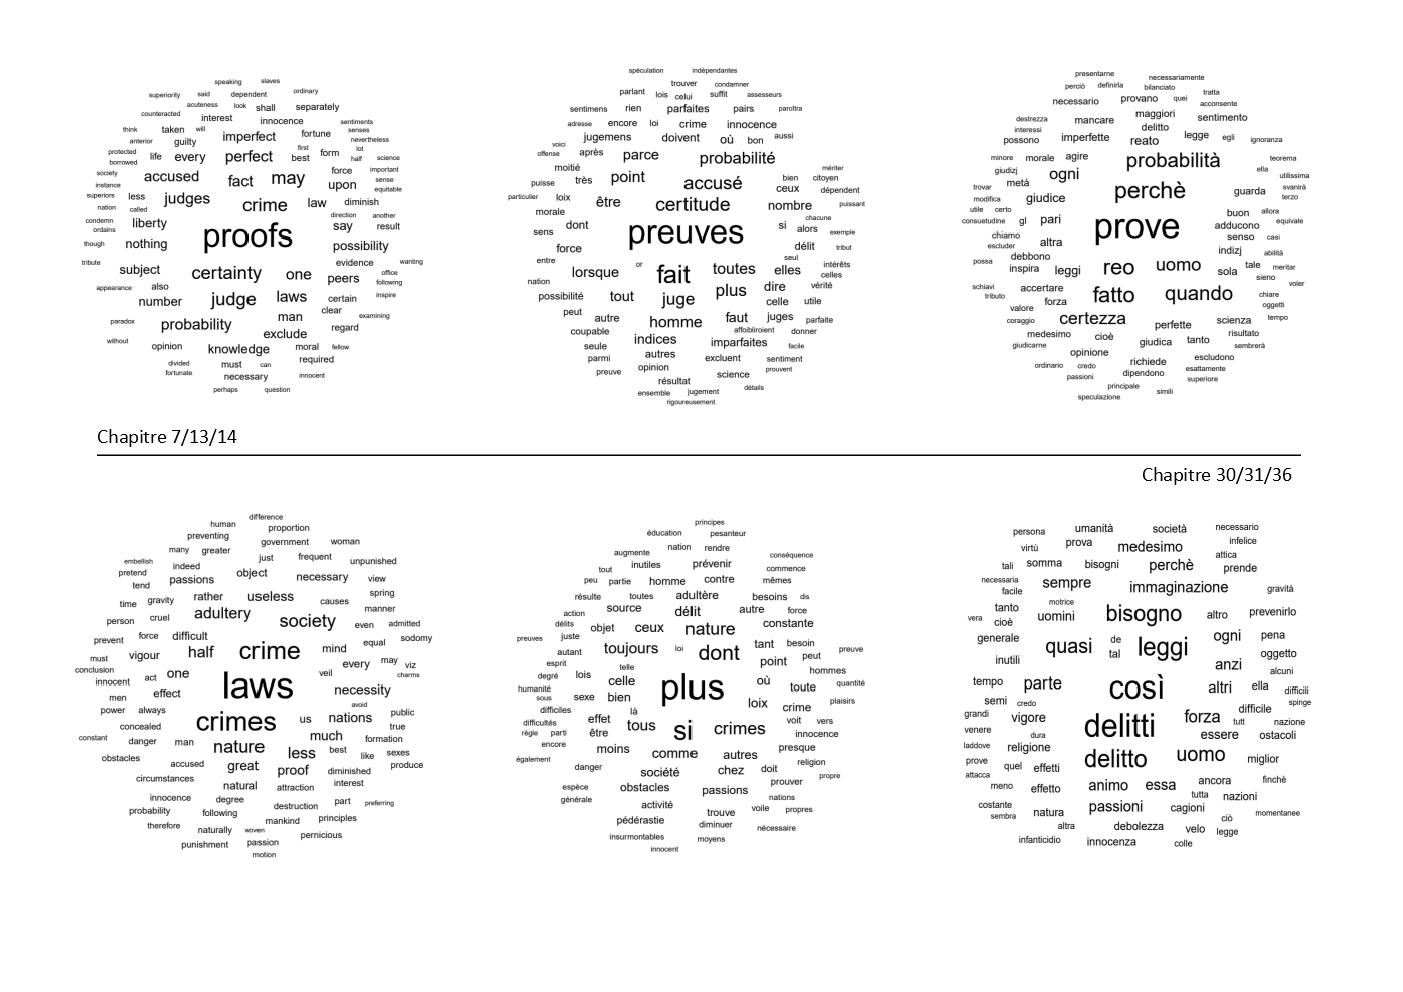
\includegraphics[width=16cm]{Partie3/images/chap3/wordcloud.jpg}}
    \caption{Nuage de mots des chapitres 7/13/14 et 30/31/36 pour les éditions anglaises, françaises et italiennes}
    \label{fig:word_cloud}
\end{figure}
Le parallèle entre les nuages de mots de ces deux chapitres est intéressant, puisque nous pouvons explicitement remarquer une différence entre les deux, simplement avec le mot le plus fréquent entre les chapitres. 

Dans la première ligne qui contient les textes du chapitre 7/13/14 dans la figure \ref{fig:word_cloud}, nous pouvons distinguer que le mot \textit{preuve} est le plus utilisé quelle que soit la langue et la taille du mot pour chacun semble montrer que la fréquence est quasiment la même qu'importe la version. Il y a donc une certaine homogénéité pour ce chapitre, comme cela peut se voir également pour les mots également très similaires qui gravitent autour de \textit{preuve}. Il est possible de citer \textit{certitude}, \textit{probabilité}, \textit{fait} ou \textit{homme} bien que ce dernier mot soit moins présent que les autres. De même pour des mots de taille moins conséquente dans le nuage, le vocabulaire est très similaire en fonction des versions. Cela laisse à penser que dans le cas de ce chapitre, il y a eu une traduction assez fidèle entre les éditions, offrant donc des nuages de mots très semblables.

À l'inverse, cette homogénéité ne se retrouve pas du tout pour le chapitre 30/31/36 sur la deuxième ligne de la même figure. Le mot le plus important n'est le même pour aucun des cas, bien que cela soit en partie dû à \textsc{rstudio}. Si les mots-vides ont effectivement été supprimés, les nuages de mots pour le chapitre en français et en italien montrent comme terme ayant la fréquence la plus importante respectivement \textit{plus} et \textit{così}\footnote{Traduction française : si}. Bien qu'il soit possible que la présence conséquente de ces mots indique un sens particulier du chapitre, celui-ci n'est pas assez explicite pour l'étude que nous effectuons et cela semble plutôt fausser le résultat du nuage. Cependant, si nous enlevons dans notre réflexion ces mots pour retrouver des termes plus éloquents, l'homogénéité n'est toujours pas présente. Le mot le plus utilisé est~: \textit{laws} pour l'anglais, \textit{nature} ou \textit{crimes} pour le français et \textit{delitti} pour l'italien. Nous sommes dans un champ lexical proche si nous considérons que \textit{crimes} est le plus utilisé en français, champ lexical qui semble d'ailleurs suivre les mots contenus dans la liste de termes définie dans le chapitre précédent et il est possible d'expliquer ce résultat. Bien que \textit{loi} ne soit pas le plus utilisé pour le français et l'italien, il reste tout de même un mot important dans ce chapitre. Nous pouvons observer que \textit{leggi} est d'une taille plutôt conséquente dans le nuage de mot de l'italien. Le cas du français est plus particulier en raison d'une différence d'orthographe~: loi s'écrit de trois manières dans les éditions françaises du corpus, \textit{loi} au singulier, \textit{lois} et \textit{loix} au pluriel. Nous pouvons distinguer deux de ces versions à une taille relativement visible dans le nuage de mots. En étudiant le reste, nous pouvons remarquer que les mots en périphérie ne montrent pas non plus une harmonie entre les versions. Cela peut nous permettre de conclure que, si le chapitre a effectivement le même sujet, qu'importe la langue, les traducteurs ont adapté leur vocabulaire et celui-ci ne correspond pas à une traduction littérale. 

Cette étude comparative entre deux chapitres nous montre donc des différences majeures entre les deux et cela peut nous laisser supposer que les traducteurs ont pris plus de libertés, dans leur vocabulaire, lors de l'édition des chapitres 30/31/36 en français et anglais par rapport à l'italien, alors que pour le chapitre 7/13/14, ils semblent avoir traduit littéralement le chapitre. De plus, les différences de structures entre certaines des versions par le travail de l'abbé Morellet\index{Morellet, Andre@Morellet, André} peuvent fausser un peu plus les résultats, ce qui n'est pas le cas pour l'autre chapitre, puisque ce dernier n'a connu aucune modification sur le fond lors de la restructuration de l'édition française de 1766.

\subsubsection{Similitudes et différences selon la langue}
Nous pouvons faire une autre analyse de nuages de mots sur un nouvel extrait, bien que l'italien ne soit pas présent ici et il ne sera donc pas possible de savoir si les traducteurs ont suivi explicitement la version originale mais nous pourrons tout de même chercher à observer des similitudes entre les deux vocabulaires utilisés.
\begin{figure}[t]
    \centering
    \fbox{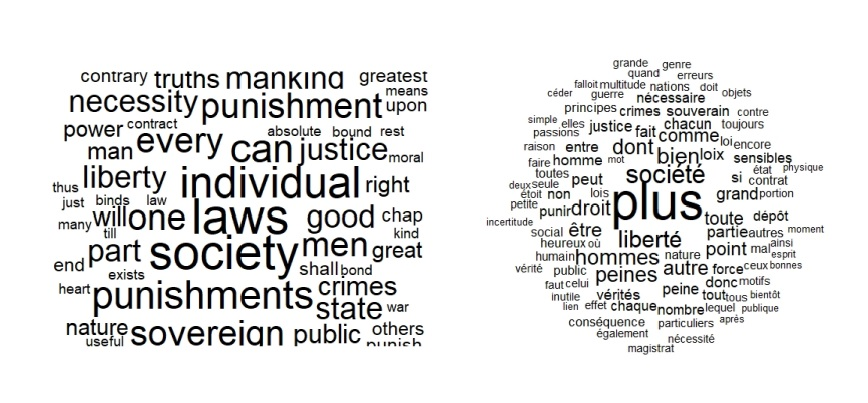
\includegraphics[width=16cm, height=8cm]{Partie3/images/chap3/wordcloud_intro.jpg}}
    \caption{Nuage de mots de la partie contenant l'introduction et les chapitres 1-2-3 pour les éditions anglaises et françaises}
    \label{fig:word_cloud_intro}
\end{figure}

En observant la figure \ref{fig:word_cloud_intro}, un élément se distingue directement~: la taille de chaque nuage de mots n'est pas équivalente. En effet, le nombre de mots maximum est de 100 et si le nuage de mots du français semble atteindre à peu près ce nombre, le nuage de mots de l'anglais semble n'en contenir que la moitié. Cela peut probablement s'expliquer par la taille des mots. En français, il y a un mot écrit largement, plusieurs mots un peu grands qui gravitent autour et d'autres mots, bien plus petits mais non de moindre importance. Dans le cas de l'anglais, nous retrouvons de très nombreux mots écrits dans une taille considérable, qui semblent prendre la majorité de l'espace du nuage de mots. En périphérie se trouve des petits mots moins présents mais non moins significatifs. L'explication du nombre de mots dans le nuage se fait par la place que prennent les mots les plus importants. Le nuage de mots est délimité par un certain espace et ainsi que l'indique \textsc{rstudio}, certains autres mots qui devaient figurer dans le nuage ne peuvent être intégrés. Cela représente une limite conséquente à cette fonctionnalité du logiciel \textsc{rstudio} mais ne crée pas de difficulté pour notre travail puisque notre intérêt ne repose que sur les mots de taille considérable. Pour le nuage de mots en français, nous avons une observation identique à celle que nous avions eu pour le chapitre 30/31/36, puisque le mot le plus fréquent est \textit{plus}. La présence de ce mot comme fréquence la plus élevée à deux reprises peut laisser supposer que \textit{plus} devrait être considéré comme un mot-vide, puisqu'il n'apporte pas d'information aux analyses et fausse le nuage de mots. En le supprimant, il serait possible de mieux discerner la place des autres mots de fréquence importante.

Une fois ces considérations prises en compte, nous pouvons comparer les nuages de mots et ce faisant, nous observons que cet extrait ne suit ni le schéma du chapitre 7/13/14, ni celui du chapitre 30/31/36. Il n'est pas homogène puisqu'il y a certains mots de taille importante dans un nuage que nous ne retrouvons pas dans l'autre mais au contraire du chapitre 30/31/36, parmi les mots importants du nuage s'observe un vocabulaire similaire tel que \textit{société/society}, \textit{loix/laws}, \textit{liberté/liberty}, \textit{souverain/sovereign}, \textit{peines/punishments}, etc. Cette comparaison nous permet également de relever que les chapitres en français semblent utiliser un lexique plus diversifié que ceux en anglais, aux vues de la différence de taille entre les mots et ce lexique traite de société, de lois et de peines, qu'importe la version.

\paragraph{}Ainsi, l'observation de ces trois chapitres différents présentés sous la forme de nuages de mots permet de nous montrer qu'il ne semble pas y avoir de réelle unité dans la manière dont sont traduits les chapitres et que les éditeurs prennent plus de libertés d'un chapitre à l'autre. Toutefois, bien que les mots ne soient pas exactement les mêmes, nous pouvons tout de même remarquer que le lexique utilisé reste similaire et cohérent en fonction des langues, laissant sa substance initiale au chapitre. Une fois ce lexique établi pour les différents chapitres que nous étudions, il sera intéressant d'analyser les liens entre ces différents mots afin de voir comment s'articule les textes.

\section{Étudier les relations de mots dans le corpus~: plusieurs méthodes pour des résultats modérément fructueux}
Élément essentiel dans les statistiques textuelles\index{Statistique textuelle}, la recherche de correspondances et de cooccurrences dans un corpus est développée grâce à de nombreux outils fournis autant par \textsc{txm} que par \textsc{r}, pour faire ressortir ces données d'une manière ou d'une autre. Cependant, même s'il existe beaucoup de méthodes, elles ne sont pas toujours concluantes ou adaptées au texte et nous allons donc observer plusieurs de ces résultats et ce qu'ils apportent ou non à notre étude.

\subsection{Explorer le texte par le biais de ses cooccurrences~: une méthode effective pour observer la structure du \emph{Traité}}
À l'aide du nuage de mots, nous avons pu observer le lexique dominant dans le corpus et les cooccurrences nous permettront de prolonger ces réflexions, puisque nous avons alors la possibilité d'observer la proximité entre ces différents mots, à savoir le vocabulaire qu'il côtoie le plus et même la manière dont s'articule le corpus. Pour réaliser cela de la meilleure manière possible, nous pourrons utiliser à la fois \textsc{r} et \textsc{txm}, qui possèdent chacun une fonctionnalité pour les cooccurrences et ces fonctionnalités peuvent se compléter pour fournir un résultat plus précis. \textsc{txm} fournit un outil simplement nommé \textbf{\textit{Cooccurrences}} qui donne la possibilité de rechercher les formes les plus proches de celle choisie pour la requête. Comme pour toutes les requêtes de \textsc{txm}, il est possible de sélectionner la propriété de la forme recherchée (mot, lemme, catégorie grammaticale, etc.) et ressortira ensuite un résultat dépendant de cette requête. Si nous nous basons sur le lexique dominant relevé avec le nuage de mots, nous choisirons donc de prendre l'option \textbf{word}. Cette recherche produit un tableau donnant la fréquence du mot de la ligne, sa co-fréquence avec le mot recherché, un indice\footnote{Indicateur statistique de présence}  et sa distance, à savoir l'écart moyen du mot vis-à-vis de l'autre mot dans la phrase, comme cela s'observe avec la figure \ref{fig:cooccurrences_preuves}. 
\begin{figure}[p]
    \centering
    \fbox{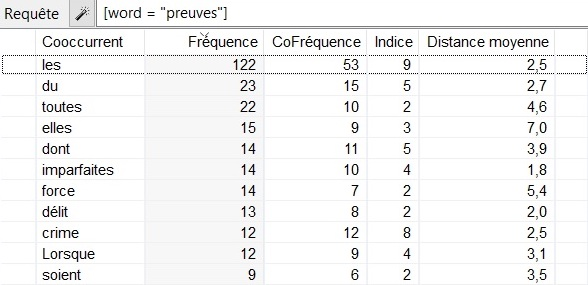
\includegraphics[width=16cm]{Partie3/images/chap3/cooccurrences_preuves.jpg}}
    \caption{Exemple du résultat sur \textsc{txm} des cooccurrences pour le mot \textit{preuves} dans le chapitre 7/13/14 dans les éditions françaises}
    \label{fig:cooccurrences_preuves}
\end{figure}
Nous avons donc, dans cette figure, un tableau de données alors que \textsc{rstudio}, tout comme pour la table lexicale, fournit ces résultats sous la forme d'un graphique, comme illustré par la figure \ref{fig:graphe_chap31}, ce qui présente des avantages et des inconvénients.
\begin{figure}[p]
    %\centering
    \fbox{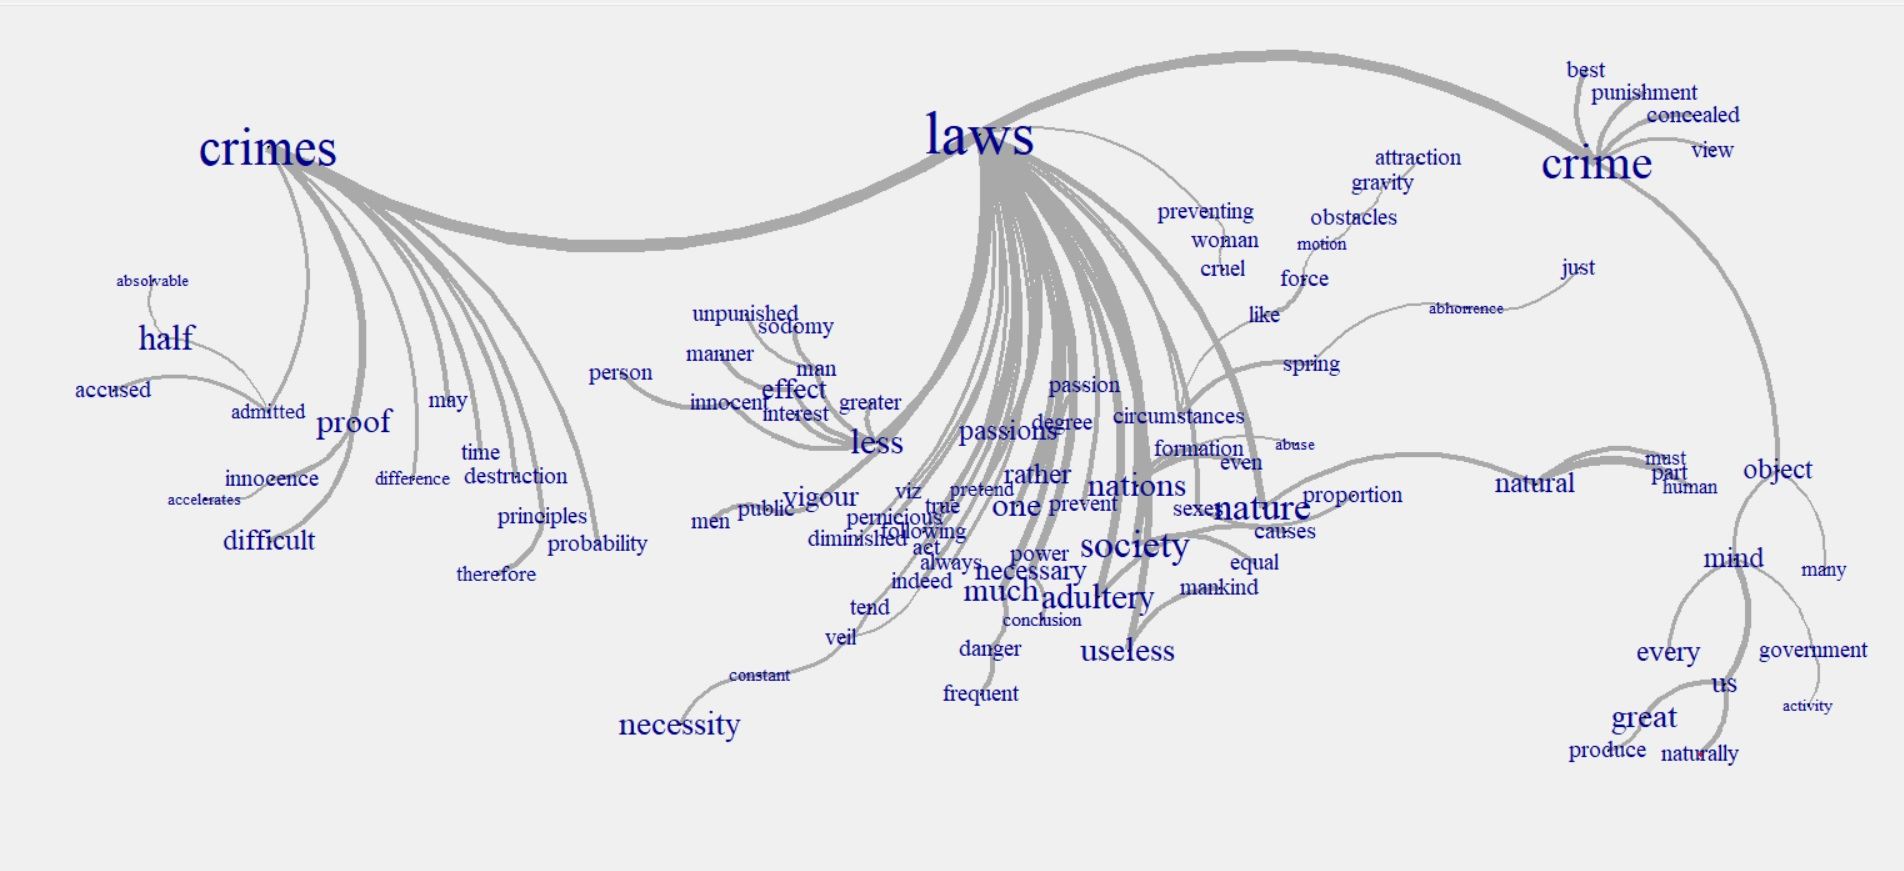
\includegraphics[width=16cm, height=10cm]{Partie3/images/chap3/graphe_chap31.jpg}}
    \caption{Graphe de mots produit par \textsc{r} représentant les cooccurrences dans le chapitre 31 des éditions anglaises}
    \label{fig:graphe_chap31}
\end{figure}
Ce graphe de mots fournit une représentation graphique de notre recherche, ce qui permet d'avoir beaucoup plus de clarté qu'avec la liste qui est produite par \textsc{txm} et de plus, les mots sont de taille différente, tout comme avec le nuage, concédant donc une véritable distinction. Cependant, ce graphe semble prendre en compte absolument tous les mots du corpus qui ne sont pas des mots-vides et donc la clarté disparaît quelque peu, comme cela s'observe pour le mot \textit{laws} dans la figure. Le mot est relié à de nombreuses autres formes mais il devient très difficile de discerner auxquelles. De manière différente, le logiciel \textsc{txm} nous indique la structure de la phrase dans son ensemble plus que ses liens entre les éléments majeurs du lexique. L'articulation entre les deux méthodes sera alors nécessaire puisque \textsc{txm} pourra compléter ce que l'aspect visuel de \textsc{rstudio} semble nous faire perdre, c'est-à-dire les données statistiques\index{Statistique textuelle} qui permettent de véritablement comprendre les liens entre les mots. Pour compléter le graphe, le principe sera donc d'aller y chercher les mots de taille assez importante et de les rechercher dans une requête \textsc{txm} pour obtenir leurs statistiques et donc avoir les chiffres exacts définissant leurs cooccurrences. En ne prenant pas en compte les mots-vides dans le tableau de résultats de \textsc{txm}, nous pouvons donc voir que les cinq co-fréquences les plus fortes avec \textit{laws} sont \textit{crime} (25), \textit{nations} (15), \textit{act} (10), \textit{pernicious} (10) et \textit{prevent} (10). Nous retrouvons ces mots dans le graphe, ce qui montre donc que les deux outils s'articulent effectivement bien ensemble. De plus, cela nous indique différents sens de l'utilisation de \textit{loi} puisque le mot semble principalement lié au terme de \textit{crime}, ce qui a du sens dans le cas du chapitre que nous étudions. Nous pouvons également observer d'autres sens, tel qu'une idée d'empêcher par les lois (\textit{prevent}) ou de les définir comme des lois d'état (\textit{nations}). \pagebreak

Il est possible d'étendre encore plus ces résultats à l'aide des concordances, que nous utiliserons plus en détails dans le chapitre suivant, concordances que nous retrouvons pour les deux logiciels mais qui seront plus claires avec \textsc{txm}. \textsc{txm} donne ici la possibilité d'envoyer les résultats de co-fréquences dans les concordances pour ainsi observer dans quelles parties du texte se placent le bout de phrases contenant les deux termes, comme cela peut se voir avec la figure \ref{fig:concordances_laws_crime}. Cette recherche de co-fréquences permet de développer notre réflexion précédente puisque nous pouvons voir que certains mots s'articulent ensemble telle une expression, comme \og~laws to prevent this crime~\fg{}. D'autres n'ont finalement pas autant de lien que la co-fréquence semblait le montrer, comme cela est représenté avec le premier résultat de la figure \ref{fig:concordances_laws_crime}. \textit{Laws} n'a aucun vrai lien avec \textit{crime}, juste une proximité entre deux phrases. 
\begin{figure}[H]
    \centering
    \fbox{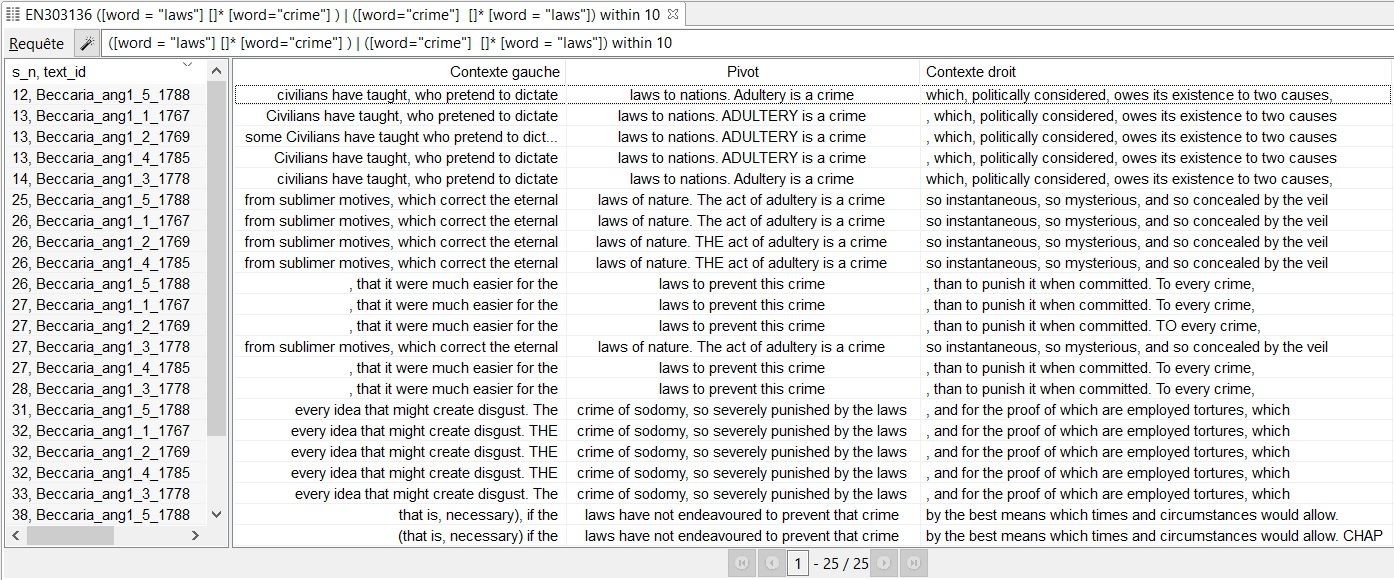
\includegraphics[width=16cm, height=9cm]{Partie3/images/chap3/concordances_laws_crime.jpg}}
    \caption{Résultats de concordances pour la recherche de cooccurrence entre \textit{crime} et \textit{laws} pour le chapitre 31 des éditions anglaises}
    \label{fig:concordances_laws_crime}
\end{figure}

\subsection{Travailler les relations à travers les correspondances~: un corpus qui ne s'approprie pas la méthode}
\textsc{txm} et \textsc{rstudio} disposent également d'autres outils pour présenter les liens du lexique, que nous appellerons ici des correspondances et que nous pourrons observer à travers une fonctionnalité~: l'\acrlong{afc}. C'est un élément très répandu en analyse statistique des données textuelles\index{Statistique textuelle} mais, comme nous le verrons, il ne sera pas adapté à notre corpus et ne donnera pas de résultats fructueux pour notre analyse. \pagebreak

Une \acrfull{afc} permet de 
\begin{quotation}
 \og~structurer l'ensemble des mots en fonction de leur répartition dans les unités textuelles. La représentation des résultats sous forme de graphique [\dots] permet de visualiser la proximité des mots, les oppositions, les tendances\footcite[p.~19]{stat_text_garnier}~\fg{}.
\end{quotation}
 L'intérêt sera donc d'observer des cooccurrences de mots et de mettre en évidence des thèmes et des oppositions de thèmes. Deux éléments de notre corpus justifient le fait que cet outil n'est pas adapté pour notre analyse. Tout d'abord, le corpus n'est pas assez long pour faire ressortir des données utiles. Même si le corpus est composé d'un certain nombre de textes, ces textes ne font chacun qu'environ quatre à six pages, ce qui ne permet pas une étude avancée et la répétition du vocabulaire apporte donc un lexique trop limité pour que cela soit intéressant. Ensuite, la spécificité même du corpus, qui est une répétition du même texte à chaque fois, avec seulement des changements mineurs, indique que cela ne sera pas productif. Le thème sera le même puisque le lexique est, comme nous l'avons vu, très juridique et les changements d'écriture d'un mot n'apporteront que des différences minimes.
\begin{figure}[p]
    \centering
    \fbox{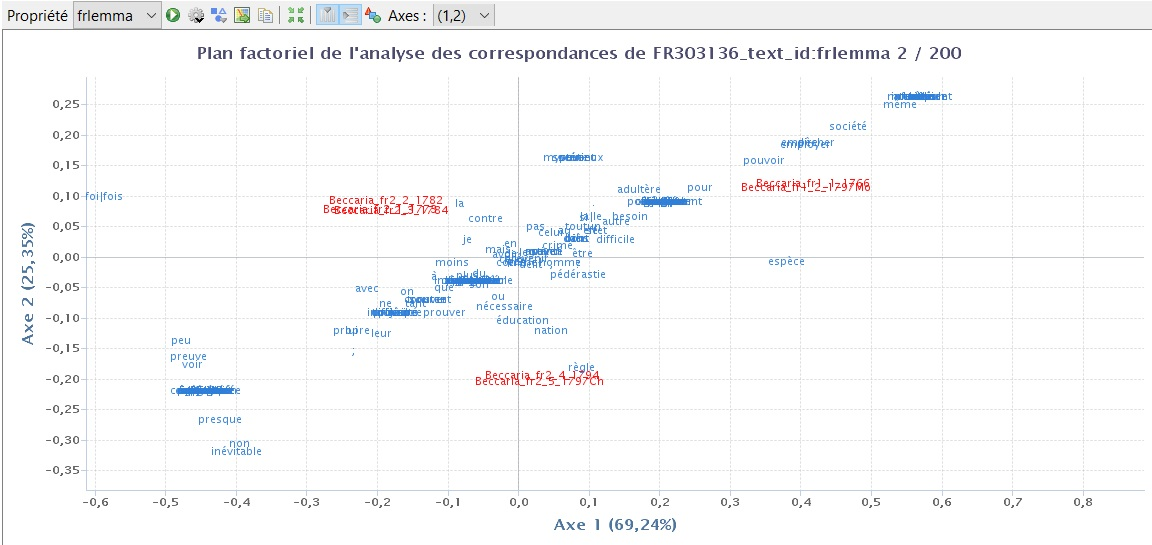
\includegraphics[width=16cm, height=10cm]{Partie3/images/chap3/afc_fr.jpg}}
    \caption{\acrshort{afc} pour le chapitre 30/31/36 des éditions françaises en prenant comme propriété le lemme}
    \label{fig:afc_fr}
\end{figure}
\begin{figure}[p]
    \centering
    \fbox{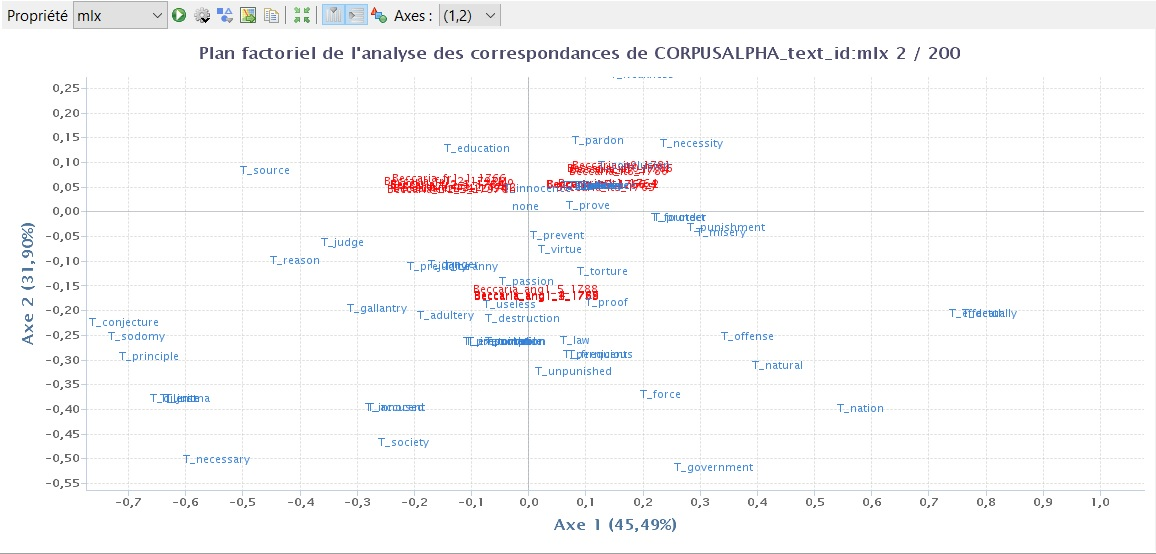
\includegraphics[width=16cm, height=10cm]{Partie3/images/chap3/afc_mlx.jpg}}
    \caption{\acrshort{afc} pour le corpus multilingue\index{Alignement!corpus multilingue} avec comme propriété l'identifiant par termes (mlx)}
    \label{fig:afc_mlx}
\end{figure}
Nous pouvons démontrer ce que nous venons d'expliquer par le biais de deux figures qui présentent deux \acrshort{afc} pour deux types d'analyse du corpus. La figure \ref{fig:afc_fr} montre une \acrshort{afc} pour le chapitre 30/31/36 des éditions françaises avec comme propriété le \textbf{frlemma} tandis que la figure \ref{fig:afc_mlx} montre le corpus multilingue\index{Alignement!corpus multilingue} avec le \textbf{mlx} en propriété. La figure \ref{fig:afc_mlx} semble de base non adaptée par la séparation observée entre les textes~: il y a trois groupes, qui sont chacun des groupes de langues du corpus. Les correspondances ne semblent pas dues tant à des cooccurrences qu'à une proximité linguistique qui influe sur le graphique. Dans le cas de la figure \ref{fig:afc_fr}, nous pouvons également observer trois groupes de textes, qui font référence aux changements mineurs que nous avons évoqué plus tôt, soit les textes structurés par Morellet\index{Morellet, Andre@Morellet, André}, les textes les plus récents avec l'écriture modernisée et le reste des éditions françaises. Les places des termes dans l'une ou l'autre des \acrshort{afc} ne paraissent pas non plus nous fournir de nouveaux éléments puisque pour discerner des thèmes, cela nécessiterait un semblant d'ordre. Ici, nous remarquons pour la figure \ref{fig:afc_fr} une diagonale formée par les lemmes qui se suivent sans discernement et pour la figure \ref{fig:afc_mlx}, il y a un éclatement de tous les \emph{mlx}, avec seulement deux ou trois groupes parfois, ce qui ne nous apporte aucun élément véritablement concret pour notre analyse.

Ainsi, ces deux exemples permettent de démontrer effectivement que les correspondances ne sont pas un moyen efficace et adapté à notre corpus actuel. Elles pourraient être plus utiles dans un cas où l'examen du texte se fait sur l'ouvrage en entier et non juste sur un chapitre précis, puisqu'il pourrait être possible, dans ce cas-là, de discerner plus de groupes de mots, grâce à un vocabulaire plus étendu et plus fourni. \pagebreak

\paragraph{}Cette exploration du corpus nous permet donc de découvrir qu'il existe de nombreux moyens pour effectuer une analyse statistique des données textuelles\index{Statistique textuelle}. Il existe plusieurs logiciels pour cela, qui disposent chacun de nombreux outils pour mener à bien l'étude selon la forme que nous voulons qu'elle prenne. Chacun de ces logiciels possède des caractéristiques propres qui leur permettent d'être plus efficace dans certains cas et surtout plus adapté aux recherches. Nous avons également pu voir que tous les modes de recherches ne sont pas adaptés en fonction du corpus. Dans notre cas, \textsc{txm} et \textsc{rstudio} présentaient chacun des avantages et des inconvénients en fonction de la recherche effectuée et pour la suite de notre travail, ce sera \textsc{txm} qui présentera la meilleure disposition pour mener à bien l'alignement\index{Alignement}, grâce à une méthode que nous avons, pour l'instant, à peine utilisée mais qui sera essentielle pour notre projet~: le concordancier\index{Concordancier}.  